\setAuthor{Marko Tsengov}
\setRound{lahtine}
\setYear{2022}
\setNumber{G 10}
\setDifficulty{10}
\setTopic{TODO}

\prob{Hantel ja pöörlemine}
\begin{wrapfigure}{r}{0.45\textwidth}
\raisebox{0pt}[\dimexpr\height-0.6\baselineskip\relax]{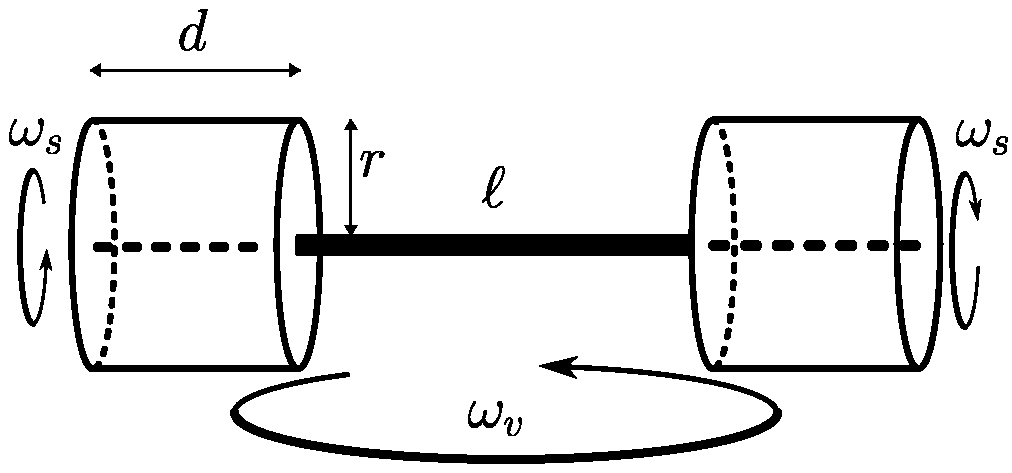
\includegraphics[scale=0.37]{2022-lahg-10-yl.pdf}}
\vspace{-15pt}
\end{wrapfigure}
Hantel koosneb kahest ühesugusest silindrist raadiusega $r$ ning kõrgusega $d$, mis on ühendatud koaksiaalselt vardaga pikkusega $l$. Varda sees on mootor, mis pöörab silindreid varda suhtes võrdsete ja vastassuunaliste nurkkiirustega $\pm \omega_s$. Millise püsiva nurkkiiruse $\omega_v$ omandab varras, kui hantel asetatakse siledale horisontaalpinnale? Eeldada, et varras ei hakka pöörlema ümber oma telje (nt saab seda takistada kinnitades varda keskkohast alla rippuva lisaraskuse).


\hint

\solu
Lahendus: vaatleme hõõrdejõust tekkivat jõumomenti hantli keskpunkti suhtes. Sümmeetria tõttu on mõlema raskuse tekitatud jõumoment $M$ sama, seega selleks, et nurkkiirendus oleks $0$, peab see jõumoment olema samuti $M = 0$.

Hantel pöörleb keskpunktist kaugusel $R$ joonkiirusega $v(R) = R \cdot \omega_v$, raskuse maad puudutav pind joonkiirusega $v_r = r \cdot \omega_s$. Normaaljõud on jaotunud ühtlaselt üle kokkupuutepinna maaga, seega on ka liugehõõrdejõu magnituud igas punktis sama ($\mu N \frac{dR}{d}$). Samas, kui $v > v_r$, on hõõrdejõud selles punktis suunatud hantli pöörlemise vastu. Juhul $v < v_r$ aga on hõõrdejõud suunatud pöörlemisega kaasa.

Eeldame, et $v > v_r$ parajasti siis, kui $R > k$. Olgu normaaljõud $N$ ning hõõrdetegur $\mu$ Sellisel juhul
\begin{gather*}
    M = \int\limits_{\ell / 2}^{k} \mu N R \frac{dR}{d} - \int\limits_{k}^{\ell/2 + d} \mu N R \frac{dR}{d} \\
    M = \frac{\mu N}{d} \left ( \int\limits_{\ell / 2}^{k} R \cdot dR - \int\limits_{k}^{\ell/2 + d} R \cdot dR \right ) \\
    0 = \frac{\mu N}{2 d} \left ( k^2 - \left ( \frac{\ell}{2} \right )^2 - \left ( \frac{\ell}{2} + d \right )^2 + k^2 \right ) \\
    0 = 2 k^2 - \frac{\ell^2}{2} - \ell d - d^2 \\
    k = \frac{1}{2} \sqrt{\ell^2 + 2 \ell d + 2 d^2} \\
    \left ( k = \sqrt{\frac{\left ( \frac{\ell}{2}\right )^2 + \left ( \frac{\ell}{2} + d \right )^2}{2}}\right )
\end{gather*}

$k$ tingimusest peab $v_r = v(k)$, seega
\begin{gather*}
    r \cdot \omega_s = k \cdot \omega_v \\
    \omega_v = \omega_s \frac{r}{k} = \omega_s \frac{2r}{\sqrt{\ell^2 + 2 \ell d + 2 d^2}}
\end{gather*}
\probend